% Use the following line _only_ if you're still using LaTeX 2.09.
%\documentstyle[icml2014,epsf,natbib]{article}
% If you rely on Latex2e packages, like most modern people use this:
\documentclass{article}

% use Times
\usepackage{times}
% For figures
\usepackage{graphicx} % more modern
%\usepackage{epsfig} % less modern
\usepackage{subfigure} 

% For citations
\usepackage{natbib}

% For algorithms
\usepackage{algorithm}
\usepackage{algorithmic}

% As of 2011, we use the hyperref package to produce hyperlinks in the
% resulting PDF.  If this breaks your system, please commend out the
% following usepackage line and replace \usepackage{icml2014} with
% \usepackage[nohyperref]{icml2014} above.
\usepackage{hyperref}

% Packages hyperref and algorithmic misbehave sometimes.  We can fix
% this with the following command.
\newcommand{\theHalgorithm}{\arabic{algorithm}}

% Employ the following version of the ``usepackage'' statement for
% submitting the draft version of the paper for review.  This will set
% the note in the first column to ``Under review.  Do not distribute.''
\usepackage{format/icml2014} 
% Employ this version of the ``usepackage'' statement after the paper has
% been accepted, when creating the final version.  This will set the
% note in the first column to ``Proceedings of the...''
%\usepackage[accepted]{icml2014}

\usepackage{times}
\usepackage{hyperref}
\usepackage{url}
\usepackage{color}
\usepackage{preamble}
\definecolor{mydarkblue}{rgb}{0,0.08,0.45}
\hypersetup{ %
    pdftitle={},
    pdfauthor={},
    pdfsubject={},
    pdfkeywords={},
    pdfborder=0 0 0,
    pdfpagemode=UseNone,
    colorlinks=true,
    linkcolor=mydarkblue,
    citecolor=mydarkblue,
    filecolor=mydarkblue,
    urlcolor=mydarkblue,
    pdfview=FitH}
    
    
\usepackage{amsmath, amsfonts, bm, lipsum, capt-of}
\usepackage{natbib, xcolor, wrapfig, booktabs, multirow, caption}
\DeclareCaptionType{copyrightbox}
\usepackage{float}

%\renewcommand{\baselinestretch}{0.99}

\def\ie{i.e.\ }
\def\eg{e.g.\ }
\let\oldemptyset\emptyset
\let\emptyset\varnothing

%\author{
%James Robert Lloyd\\
%University of Cambridge\\
%Department of Engineering\\
%\texttt{jrl44@cam.ac.uk}
%\And
%David Duvenaud\\
%University of Cambridge \\
%Department of Engineering \\
%\texttt{dkd23@cam.ac.uk}
%\And
%Roger Grosse\\
%M.I.T.\\
%Brain and Cognitive Sciences \\
%\texttt{rgrosse@mit.edu}
%\And
%Joshua B. Tenenbaum\\
%M.I.T.\\
%Brain and Cognitive Sciences \\
%\texttt{jbt@mit.edu}
%\And
%Zoubin Ghahramani\\
%University of Cambridge \\
%Department of Engineering \\
%\texttt{zoubin@eng.cam.ac.uk}
%}

\newcommand{\fix}{\marginpar{FIX}}
\newcommand{\new}{\marginpar{NEW}}

\setlength{\marginparwidth}{0.6in}
%%%%%%%%%%%%%%%%%%%%%%%%%%%%%%%%%%%%%%%%%%%%%%%%%%%%%%%%%%
%%%% EDITING HELPER FUNCTIONS  %%%%%%%%%%%%%%%%%%%%%%%%%%%
%%%%%%%%%%%%%%%%%%%%%%%%%%%%%%%%%%%%%%%%%%%%%%%%%%%%%%%%%%

%% NA: needs attention (rough writing whose correctness needs to be verified)
%% TBD: instructions for how to fix a gap ("Describe the propagation by ...")
%% PROBLEM: bug or missing crucial bit 

%% use \fXXX versions of these macros to put additional explanation into a footnote.  
%% The idea is that we don't want to interrupt the flow of the paper or make it 
%% impossible to read because there are a bunch of comments.

%% NA's (and TBDs, those less crucially) should be written so 
%% that they flow with the text.

\definecolor{WowColor}{rgb}{.75,0,.75}
\definecolor{SubtleColor}{rgb}{0,0,.50}

% inline
\newcommand{\NA}[1]{\textcolor{SubtleColor}{ {\tiny \bf ($\star$)} #1}}
\newcommand{\LATER}[1]{\textcolor{SubtleColor}{ {\tiny \bf ($\dagger$)} #1}}
\newcommand{\TBD}[1]{\textcolor{SubtleColor}{ {\tiny \bf (!)} #1}}
\newcommand{\PROBLEM}[1]{\textcolor{WowColor}{ {\bf (!!)} {\bf #1}}}

% as margin notes

\newcounter{margincounter}
\newcommand{\displaycounter}{{\arabic{margincounter}}}
\newcommand{\incdisplaycounter}{{\stepcounter{margincounter}\arabic{margincounter}}}

\newcommand{\fTBD}[1]{\textcolor{SubtleColor}{$\,^{(\incdisplaycounter)}$}\marginpar{\tiny\textcolor{SubtleColor}{ {\tiny $(\displaycounter)$} #1}}}

\newcommand{\fPROBLEM}[1]{\textcolor{WowColor}{$\,^{((\incdisplaycounter))}$}\marginpar{\tiny\textcolor{WowColor}{ {\bf $\mathbf{((\displaycounter))}$} {\bf #1}}}}

\newcommand{\fLATER}[1]{\textcolor{SubtleColor}{$\,^{(\incdisplaycounter\dagger)}$}\marginpar{\tiny\textcolor{SubtleColor}{ {\tiny $(\displaycounter\dagger)$} #1}}}


%% For submission, make all render blank.
%\renewcommand{\LATER}[1]{}
%\renewcommand{\fLATER}[1]{}
%\renewcommand{\TBD}[1]{}
%\renewcommand{\fTBD}[1]{}
%\renewcommand{\PROBLEM}[1]{}
%\renewcommand{\fPROBLEM}[1]{}
%\renewcommand{\NA}[1]{#1}  % Note, NA's pass through!


% The \icmltitle you define below is probably too long as a header.
% Therefore, a short form for the running title is supplied here:
\icmltitlerunning{Using kernel two sample tests for statistical-model checking}

\begin{document} 

\twocolumn[
\icmltitle{Using kernel two sample tests for statistical-model checking}

% It is OKAY to include author information, even for blind
% submissions: the style file will automatically remove it for you
% unless you've provided the [accepted] option to the icml2014
% package.
\icmlauthor{Your Name}{email@yourdomain.edu}
\icmladdress{Your Fantastic Institute,
            314159 Pi St., Palo Alto, CA 94306 USA}
\icmlauthor{Your CoAuthor's Name}{email@coauthordomain.edu}
\icmladdress{Their Fantastic Institute,
            27182 Exp St., Toronto, ON M6H 2T1 CANADA}

% You may provide any keywords that you 
% find helpful for describing your paper; these are used to populate 
% the "keywords" metadata in the PDF but will not be shown in the document
\icmlkeywords{}

\vskip 0.3in
]

\begin{abstract} 
We invetigate the utility of the maximum mean discrepancy two sample test as a means of statistical model assessment.
We apply it to several unsupervised learning models and investigate their inaccuracies.
\end{abstract} 

\allowdisplaybreaks

\section{Introduction}

\TBD{Model checking or model assessment? Gelman et amici use 'checking'}

Model assessment or checking is an inevitable component of a complete data analysis.
It is going to be especially important as probabilistic programming takes off and people build complicated custom models.

Usually one chooses statistics of interest and evaluates the extent to which the beliefs of the model and realised value on the data align.
But how does one generate these statistics?
Ideally one chooses statistics that are of practical importance.

However, it would also be interesting to find the statistic that most strongly indicates a discrepancy; enter MMD.

Call to arms about a lack of model checking in machine learning literature - find some quotes where new models come from speculations about the form of data.

\section{Background: Model checking via posterior predictive $p$-values}

Suppose we observe data $Y = (y_i)_{i=1\ldots n}$ and we attempt to fit a model $M$ with parameters $\theta$.
After performing a statistical analysis we will have either an estimate, $\hat\theta$, or an (approximate) posterior, $p(\theta|M,Y)$, for the parameters.

The posterior predictive distribution over replicate data $Y^\textrm{rep}$ is given by
\begin{equation}
p(Y^\textrm{rep}|M,Y) = \int p(Y^\textrm{rep}|M,\theta)p(\theta|M,Y)\mathrm{d}\theta
\end{equation}
where the posterior distribution for $\theta$ is replaced by a delta function in a frequentist analysis.
In a Bayesian context this represents the belief over potential future data sets generated by the same mechanism as the first data set.

Posterior predictive $p$-values (cite Rubin 1984, Meng 1994, Gelman 1996) are defined by\fTBD{check notation is up to date}
\begin{equation}
p_b(Y) = \mathbb{P}(T(Y^\textrm{rep})\geq T(Y)|M,Y)
\end{equation}
where $T$ is a statistic \ie a function of the data.
This is the posterior probability that a potential future data set will be more extreme than the observed data as measured by the statistic $T$.
Small $p$-values indicate that the observed data is extreme compared to the posterior predictive distribution, indicating a lack of fit between the posterior distribution and the data.

\TBD{Alternatively it can be related to an estimate of utility of a model for predicting a certain quantity - I think - at least some Swedes claim this.}

For example, if $T$ is the sample skewness\fTBD{Worth including? Actually show a synthetic data example?}
\begin{equation}
T(Y) = \frac{\frac{1}{n}\sum (y_i-\bar y)^3}{\big(\frac{1}{n}\sum (y_i- \bar y)^2\big)^{3/2}}
\end{equation}
then a small $p$-value based on this statistic would indicate that the data was more positively skewed than expected by the posterior predictive distribution.
This would happen if \eg one tried to model positively skewed data using a symmetric distribution.

In practice, statistics are chosen to measure aspects of the data that are of relevance to the analysis being performed.
Whilst there are numerous examples (cite some applied papers) of sensible choices for standard models, there is little work on exploratory model assessment.

\section{Background: Maximum mean discrepancy}

Consider the two sample problem \ie given samples $X = (x_i)_{i=1\ldots m}$ and $Y = (y_i)_{i=1\ldots n}$ drawn \iid from distributions $p$ and $q$ respectively, can we determine if $p \neq q$?

This can be answered by considering maximum mean discrepancy (MMD) (cite Gretton) statistics (also called integral probability metrics by Mueller 1997)
\begin{equation}
\textrm{MMD}(\mathcal{F},p,q) = \sup_{f \in \mathcal{F}}(\mathbb{E}_{x\sim p}[f(x)] - \mathbb{E}_{y\sim q}[f(y)])
\end{equation}
where $\mathcal{F}$ is a set of functions.
These types of statistics are of interest since they are computed at the function that extremises the discrepancy between two distributions, subject to the constraints of the function space $\mathcal{F}$.

When $\mathcal{F}$ is a reproducing kernel Hilbert space (RKHS) the function attaining the supremum can be derived analytically and is called the witness function
\begin{equation}
f(x) = \mathbb{E}_{x'\sim p}[k(x,x')] - \mathbb{E}_{x'\sim q}[k(x,x')]
\end{equation}
where $k$ is the kernel of the RKHS.
Consequently the MMD can be expressed without the supremum as
\begin{eqnarray}
\textrm{MMD}^2(\mathcal{F},p,q) & = & \phantom{-2}\mathbb{E}_{x,x'\sim p}[k(x,x')] \nonumber\\
&& - 2\mathbb{E}_{x\sim p,y\sim p}[k(x,y)] \nonumber\\
&& + \phantom{2}\mathbb{E}_{y,y'\sim q}[k(y,y')]
\end{eqnarray}
for which one can form a simple biased estimate\fTBD{Maybe cut equation given length}
\begin{eqnarray}
\textrm{MMD}_b^2(\mathcal{F},X,Y) & = & \phantom{+}\frac{1}{m^2}\sum_{i,j=1}^{m}k(x_i,x_j) \nonumber\\
&& - \frac{2}{mn}\sum_{i,j=1}^{m,n}k(x_i,y_j) \nonumber\\
&& + \frac{1}{n^2}\sum_{i,j=1}^{n}k(y_i,y_j)
\end{eqnarray}
with which one can construct statistical tests of whether or not $p=q$.

The witness function can be estimated from finite samples similarly
\begin{equation}
\hat{f}(x) = \frac{1}{m}\sum_{i=1}^{m}k(x,x_i) - \frac{1}{n}\sum_{i=1}^{n}k(x,y_i).
\end{equation}

From this final equation we can see that the empirical witness function is the difference of two kernel density estimates (cite Nadaraya and Watson probably).

\section{Kernel MMD for posterior predictive checking}

Posterior predictive $p$-values ask the question 'Is the data extreme compared to my posterior as measured by a particular statistic?'.
Instead we ask the question 'Is it plausible that the data could have been generated by my posterior?'; we use kernel two sample tests to answer this question.

We phrase this as a two sample problem.
Suppose we have samples $\theta_i \dist p(\theta|M,Y)$ from our (approximate) posterior distribution, either from MCMC or sampling from a fitted distribution.
We then generate replicate data
\begin{equation}
Y^\textrm{rep} = (y^\textrm{rep}_i \dist p(y^\textrm{rep}_i|M,\theta_i))_{i=1\ldots m}
\end{equation}
from the predictive distribution for each sample of the parameters.

We then ask whether or not $Y^\textrm{rep}$ and $Y$ come from the same distribution using a kernel MMD test.
The appeal of using kernel two sample tests is that we get a $p$-value determining statistical significance, but we also get an estimate of the witness function, which shows us where the two distributions differ most, allowing a more exploratory form of model checking.

In the rest of this manuscript we demonstrate how kernel MMD tests can be used to check fitted models and how the witness function can be used to identify any discrepancies between a model and data.

\subsection{Kernel choice}

Normal stuff that RBF is a common default.
Matern might be better in higher dimensions.
Fancier stuff needed for \eg string, graphs.

Lengthscale also important, discuss the median distance heuristic and other possible methods (and relation of MMD to average discrepancy under GP prior).

\subsection{Estimation of null distribution}

We use the bootstrap.
But fancier methods exist when one has lots of data (cite the latest machinery).

\paragraph{Noto bene}

\TBD{
Model checking should not replace model comparison and averaging and posterior predictive $p$-values determine \emph{statistical} significance, not \emph{practical} significance.
}

\section{Toy examples}

\subsection{Newcomb's speed of light data}

\TBD{nanseconds $\to$ nanoseconds}

A histogram of Simon Newcomb's (cite - Stigler 1977 possibly) 66 measurements used to determine the speed of light is shown in figure~\ref{fig:newcomb_hist}.
We consider fitting a normal distribution to this data by maximum likelihood\footnotemark.
\footnotetext{66 data points in one dimension is strongly informative, maximum likelihood will give very similar results to a fully Bayesian treatment with weakly informative priors}

\begin{figure}[ht]
\centering
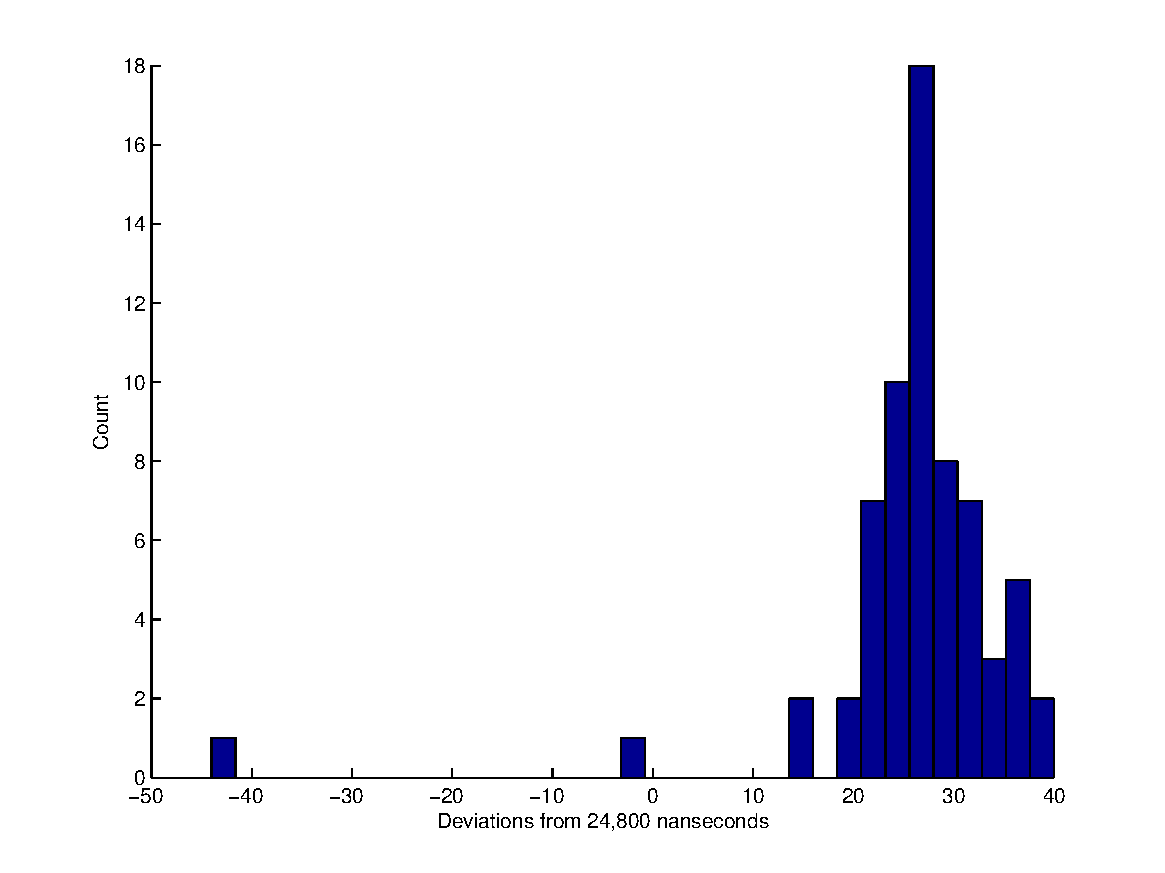
\includegraphics[width=0.98\columnwidth]{figures/newcomb_hist}
\caption{
Histogram of Simon Newcomb's speed of light measurements.
}
\label{fig:newcomb_hist}
\end{figure}

We sampled 1000 points from the fitted distribution and performed a kernel two sample test with 1000 bootstrap replications.
The estimated $p$-value of the test was less than 0.001 \ie a clear disparity between the model and data.
The data, fitted density estimate (the normal distribution) and witness function are shown in figure~\ref{fig:newcomb_witness_1}.
The witness function has a trough at the centre of the data and peaks either side.
This indicates that the fitted model has placed too little mass in its centre and too much mass outside its centre; this indicates that the data is more leptokurtic or has smaller variance than the fitted model.

\begin{figure}[ht]
\centering
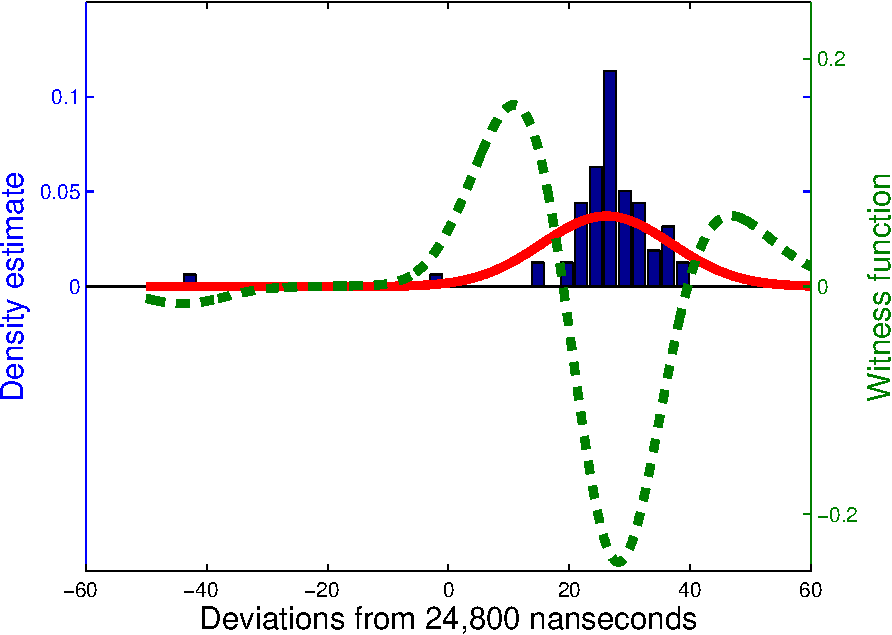
\includegraphics[width=0.98\columnwidth]{figures/newcomb_witness_1}
\caption{
Histogram of Simon Newcomb's speed of light measurements together with density estimate (red solid line) and MMD witness function (green dashed line).
}
\label{fig:newcomb_witness_1}
\end{figure}

This suggests that we should modify our model by either allowing for heavy tails or explicitly modelling the possibility of outliers (which could have resulted in the variance being over-estimated).
\TBD{
Student-$t$ with two degrees of freedom is ok-ish.
Probably will be beaten by normal + outlier model - need to check in Church or something like that.
Model check says ignoring the outliers and fitting a Gaussian is ok - $p$-value near 0.5 (plenty of bootstrap variation).
New witness function is finding smaller scale discrepancies - but model check says it's ok.
The witness function is kinda testing for asymmetry - maybe not, hard to tell.
}

\begin{figure}[ht]
\centering
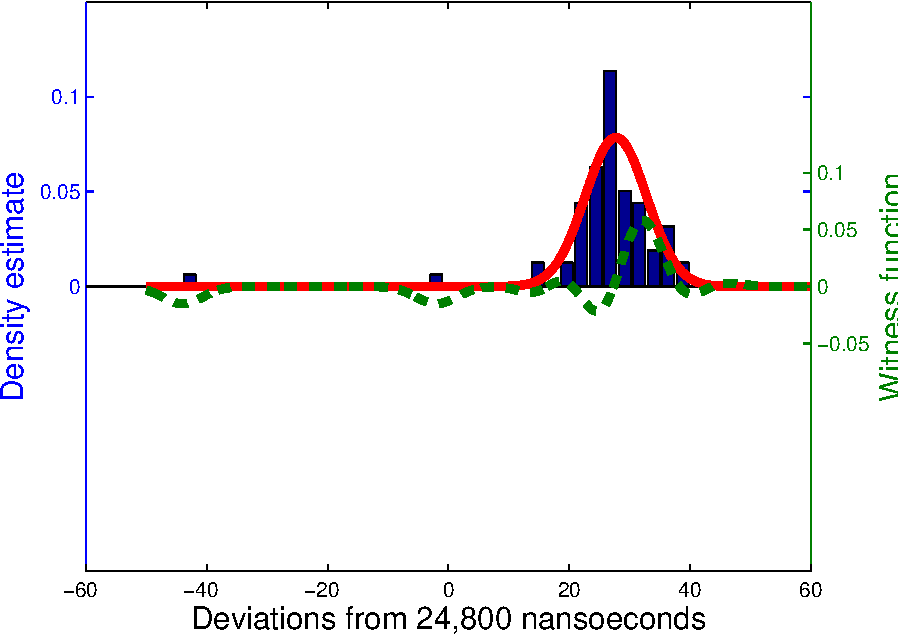
\includegraphics[width=0.98\columnwidth]{figures/newcomb_witness_2}
\caption{
Histogram of Simon Newcomb's speed of light measurements together with improved density estimate (red solid line) and MMD witness function (green dashed line).
}
\label{fig:newcomb_witness_1}
\end{figure}

\paragraph{Noto bene}
\TBD{
MMD not good for identifying outliers - tends to find dense discrepancies.
But it will flag a problem if the fitted model was not robust to outliers 
}

\subsection{Spotting an unusual cluster}

Figure~\ref{fig:blob_blob_ring} shows synthetic 2 dimensional data generated from two Gaussians and a uniform ring density (green circles).

\begin{figure}[ht]
\centering
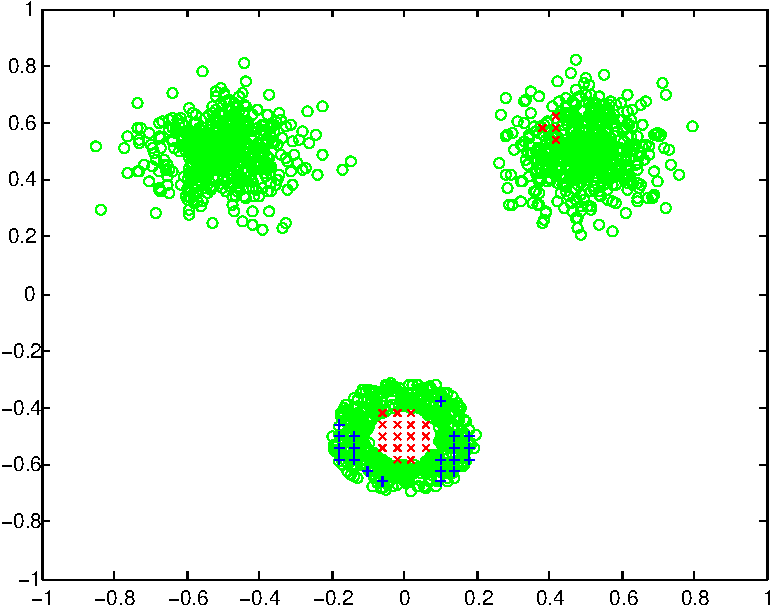
\includegraphics[width=0.98\columnwidth]{figures/blob_blob_ring}
\caption{
An experiment on synthetic data revealing a statistically significant maximum mean discrepancy.
Green $\circ$ are data, red $\times$ are locations over-represented by the model, blue $+$ are locations under-represented by the model.
}
\label{fig:blob_blob_ring}
\end{figure}

We fit a mixture of Gaussians (cite) to this data using 3 centres.
The kernel two sample test using the median lengthscale heuristic returns a $p$-value of (insert number here) indicating that no discrepancies can be identifed at this lengthscale.
However, plotting a histogram of all pairwise distances over the data reveals two predominant scales in the data; the median is closest to the larger value.

Performing a kernel two sample test with the smaller lengthscale results in a $p$-value of (insert number) indicating a discrepancy between the model and the data.
Similar to before we can identify this discrepancy via the witness function.
\TBD{
Something about extreme points or basins of attraction or a plot of the witness function.
}
The witness function has clearly identified the uniform ring of data points as being inconsistent with the mixture of Gaussians model.

\TBD{Follow up could be trying to fit this with more Gaussians - how many do we need to patch it up - will there always be discrepancies or will they become too small to notice?}

\section{Case studies}

\subsection{What exactly do neural networks dream about?}

``To recognize shapes, first learn to generate images'' \cite{Hinton2007}.
Restricted Boltzmann Machine (RBM) pretraining of neural networks was shown by \cite{Hinton2006} to learn a deep belief network (DBN) (cite) for the training data \ie a generative model.
Subsequently, as well as computing estimates of marginal likelihood and testing errors, it became standard to demonstrate the effectiveness of a neural network by generating samples from the distribution it had learned\fTBD{cite things}.

When trained on the MNIST handwritten digit data, the samples certainly look like digits, but it is hard to detect any systematic anomalies purely by visual inspection.
We now use the kernel two-sample test to investigate how faithfully RBMs and DBNs can capture the probability distribution over handwritten digits.

\subsubsection{RBMs prefer rounded numbers}

We trained an RBM with architecture $(784)\leftrightarrow(500)\leftrightarrow(10)$ using 15 epochs of PCD-15, a batch size of (something) and a learning rate of 0.1 (\ie we used the same settings as the code available at (cite deep learning tutorial)).
We generated 3000 independent samples from the learned generative model by initialising the network with a random training image and performing 1000 clamped gibbs updates (without clamping the label pixels, the generative distribution is biased towards certain digits) to generate each image (this is standard \eg \cite{Hinton2007}).

Figure~\ref{fig:rbm_samples} shows the first twenty random samples from this model.
They look like digits, but has the true distribution over digits been faithfully captured?
A priori the answer to this question is almost certainly no, but it is not immediately obvious how the learned distribution will deviate from the true distribution.

\begin{figure}[ht]
\centering
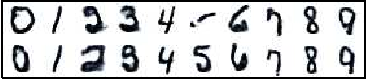
\includegraphics[width=0.98\columnwidth]{figures/rbm_samples}
\caption{
Samples from an RBM (actually the mean activations).
}
\label{fig:rbm_samples}
\end{figure}

Performing a kernel two sample test using the median length scale heuristic resulted in an estimated $p$-value less than 0.001 \ie a clear discrepancy between the model and the data.
We can investigate this discrepancy by examining the images at which the witness function is extremised.
The most over/under represented images are displayed in figure~\ref{fig:rbm_over_under}.
The RBM appears to over-represent rounded 2/3/9 whilst it under-represents slanted 3, 5 and 8.

\begin{figure}[ht]
\centering
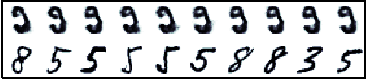
\includegraphics[width=0.98\columnwidth]{figures/rbm_over_under}
\caption{
Over (top row) and under (bottom row) represented images by the RBM.
}
\label{fig:rbm_over_under}
\end{figure}

To test that this was not just a poorly trained single RBM, we trained 1500 RBMs and generated one sample from each and performed the same tests.
The estimated $p$-value was 0.005.
We show the over/under represented images in figure~\ref{fig:many_rbm_over_under}.

\begin{figure}[ht]
\centering
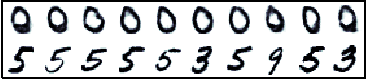
\includegraphics[width=0.98\columnwidth]{figures/many_rbm_over_under}
\caption{
Over (top row) and under (bottom row) represented images by many RBMs.
}
\label{fig:many_rbm_over_under}
\end{figure}

Again, a rounded number is over-represented whilst slanted digits are under-represented.
\TBD{
To better probe the round / slanty hypothesis further lets look at conditional distributions.
Figure~\ref{fig:many_rbm_over_under_digit} shows that the RBMs are mislabeling on average - the digits 2 and 5 are close.
}

\begin{figure}[ht]
\centering
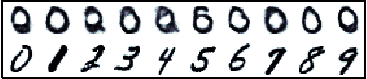
\includegraphics[width=0.98\columnwidth]{figures/many_rbm_over_under_digit}
\caption{
Over (top row) and under (bottom row) represented images by many RBMs - conditional distributions.
}
\label{fig:many_rbm_over_under_digit}
\end{figure}

\TBD{
Now separating by PCA in figure~\ref{fig:many_rbm_over_under_pca}.
It is still mostly curvy against slanty.
}

\begin{figure}[ht]
\centering
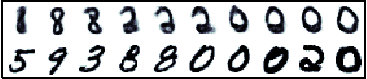
\includegraphics[width=0.98\columnwidth]{figures/many_rbm_over_under_pca}
\caption{
Over (top row) and under (bottom row) represented images by many RBMs - PCA spread.
}
\label{fig:many_rbm_over_under_pca}
\end{figure}

\TBD{
So what is going wrong?
It is probably something to do with round numbers using similar features and therefore these features get better developed faster?
}

\subsubsection{DBNs have nightmares about ghosts}

\TBD{Experimentation with fine tuning after pre-training work in progress}

\TBD{
Trained one DBN with architecture $(784)\leftarrow(500)\leftarrow(500)\leftrightarrow(2000)\leftrightarrow(10)$.
Again get a tiny $p$-value.
Here are some pictures.
}

\begin{figure}[ht]
\centering
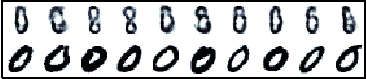
\includegraphics[width=0.98\columnwidth]{figures/dbn_over_under}
\caption{
Over (top row) and under (bottom row) represented images by DBN.
}
\label{fig:dbn_over_under}
\end{figure}

\begin{figure}[ht]
\centering
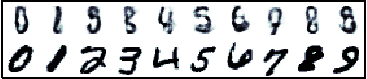
\includegraphics[width=0.98\columnwidth]{figures/dbn_over_under_digit}
\caption{
Over (top row) and under (bottom row) represented images by DBN - conditional distributions.
}
\label{fig:dbn_over_under_digit}
\end{figure}

\TBD{
The over-represented images are somewhat 'ghosted' - \ie it looks like multiple images on top of each other.
In contrast therefore the under-represented images are fat and bold.
This is prabably due to 'mistakes' in the sampling process in higher levels resulting in incorrect activations of several neurons in lower levels.
Not entirely sure how to best probe this - to be discussed.
}

\TBD{
I am currently trying to generatively fine tune the dbn using a CD algorithm proposed by Geoff Hinton - need to have a very small learning rate - work in progress.
}

\subsection{Pitman-Yor processes say the darndest things}

Look http://www.sequencememoizer.com/ and http://www.gatsby.ucl.ac.uk/~ucabjga/code.html

\section{Discussion}

Do you know what your model is up to right now?
Maybe you should check it is ok.

Can also apply to Geweke tests.

Future - graphs, functions\ldots

\bibliography{gpss, library}
\bibliographystyle{format/icml2014}

\end{document} 
